\begin{frame}{Semantic Segmentation}
  \begin{figure}
    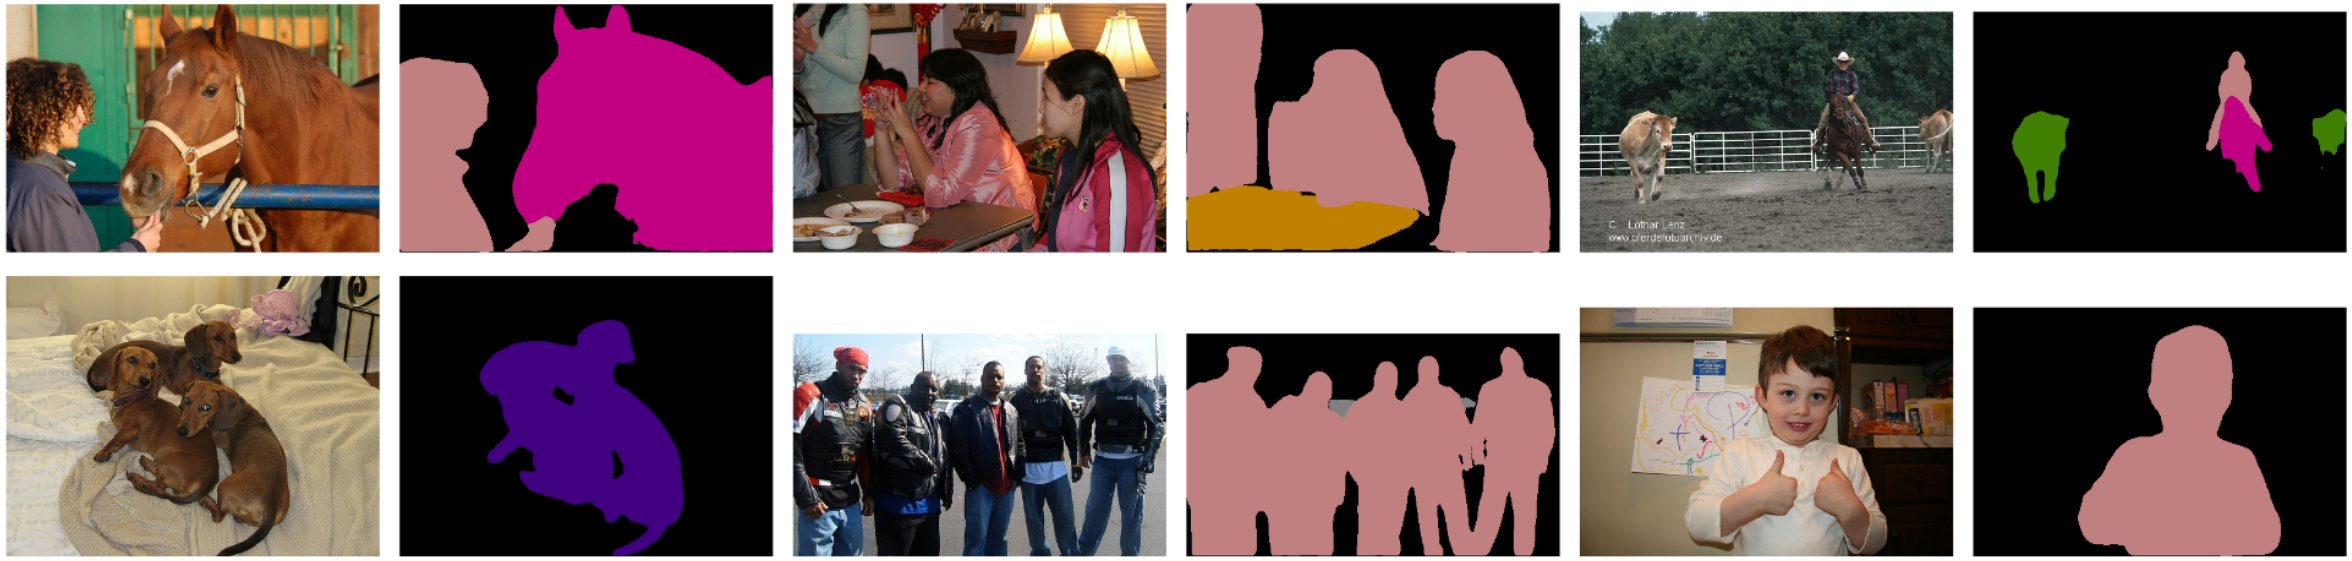
\includegraphics[width=0.9\textwidth]{deeplabv3p_result_00}
  \end{figure}
  \note{
    \begin{itemize}
      \item Semantic Segmentation is the task of classifying every pixel of an image with an object class.
      \item Often including a background class.
    \end{itemize}
  }
\end{frame}


\begin{frame}{Dataset: Cityscapes}
  \begin{columns}
    \begin{column}{0.48\textwidth}
      \begin{figure}
        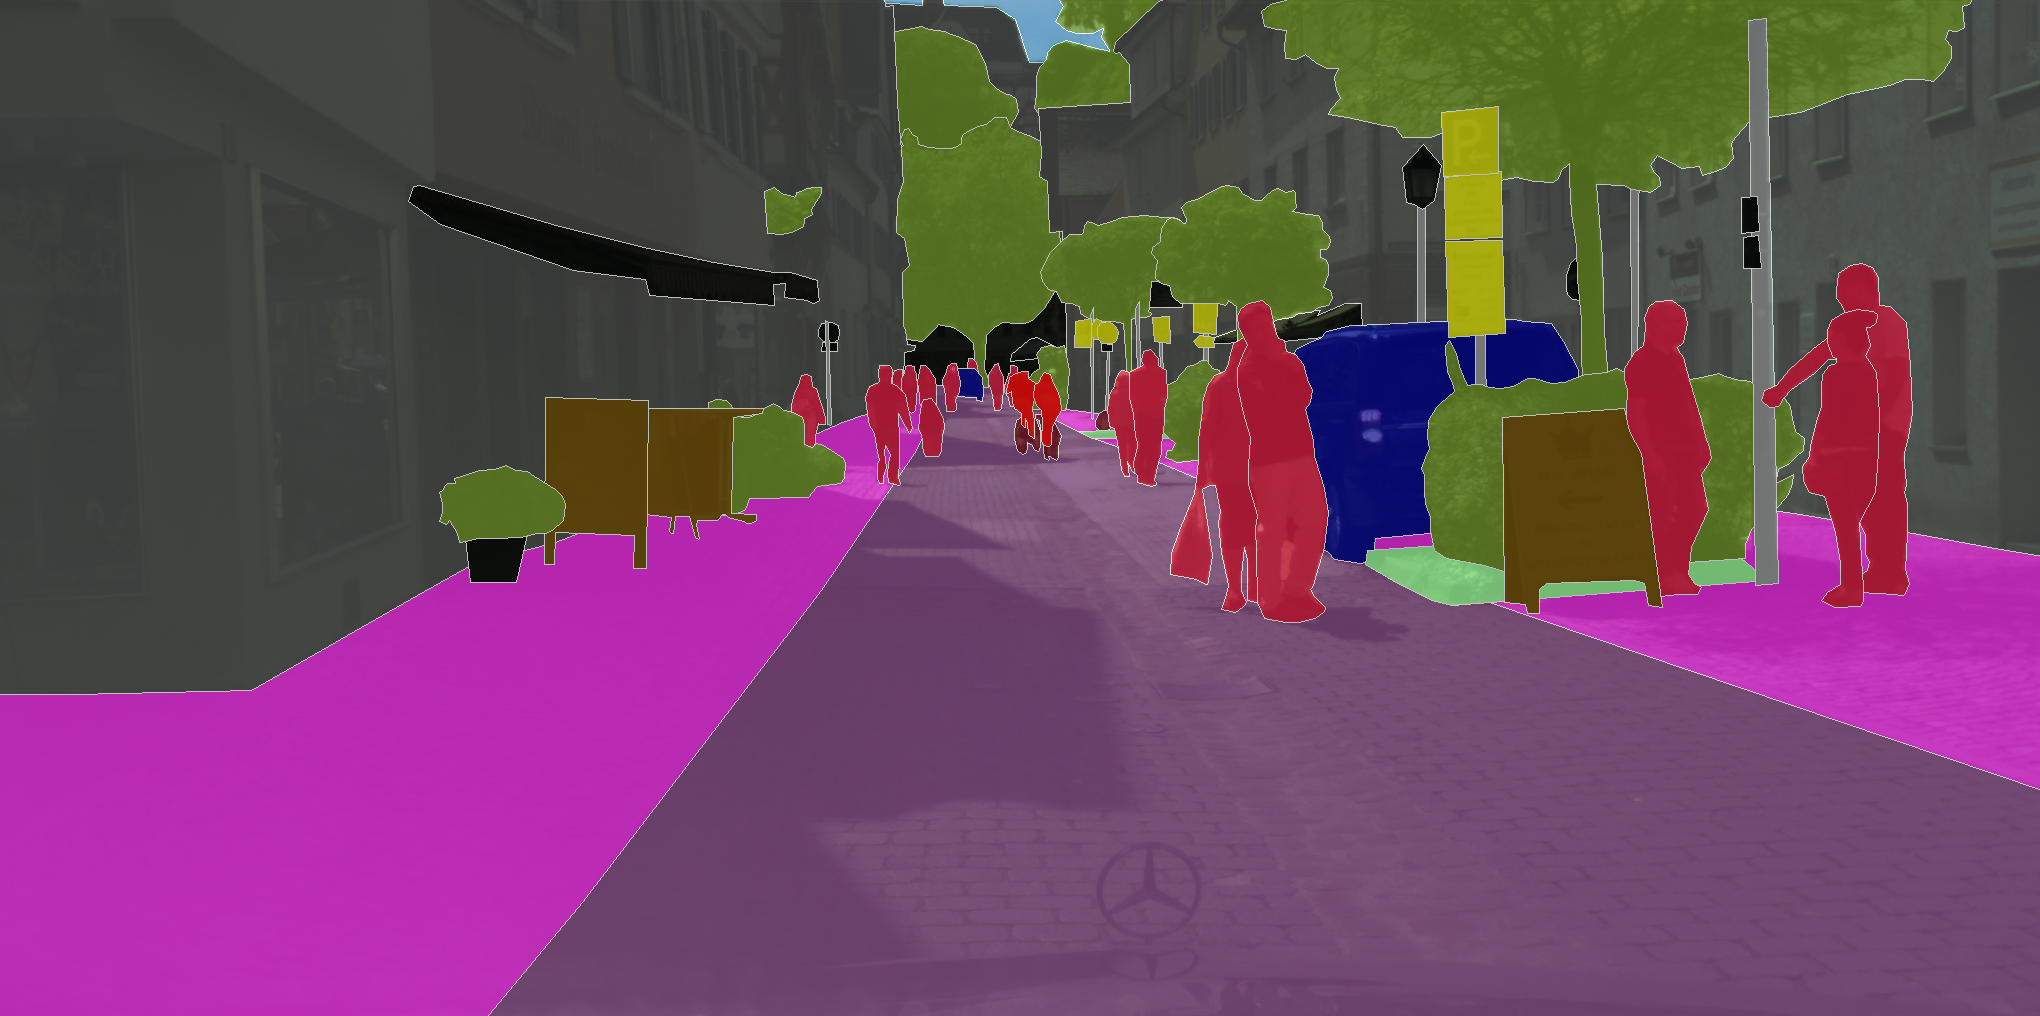
\includegraphics[width=0.9\textwidth]{segmentation_cityscape_tuebingen}
      \end{figure}
    \end{column}
    \begin{column}{0.48\textwidth}
    \begin{itemize}
      \item 30 classes
      \item 5000 annotated images with fine annotation
      \item 20000 annotated images with coarse annotations
    \end{itemize}

    \end{column}
  \end{columns}

\end{frame}


\begin{frame}{Dataset: COCO Common Objects in Context }
  \begin{columns}
    \begin{column}{0.48\textwidth}
      \begin{figure}
        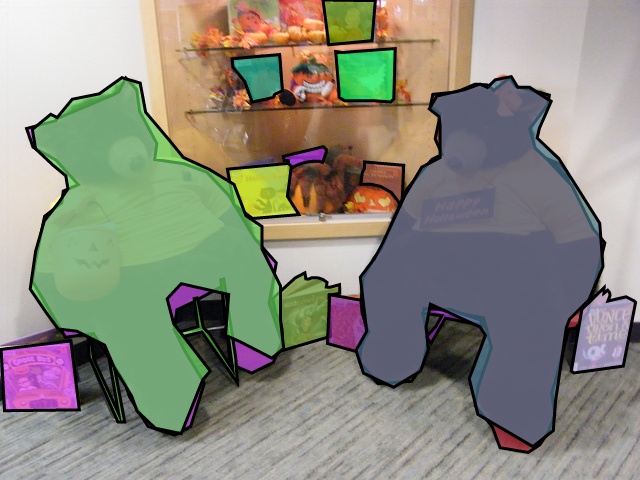
\includegraphics[width=0.9\textwidth]{segmentation_coco_bears}
      \end{figure}
    \end{column}
    \begin{column}{0.48\textwidth}
    \begin{itemize}
      \item 1.5 million object instances
      \item 80 object categories
      \item 91 stuff categories
      \item 330K images ($>$200K labeled)
    \end{itemize}

    \end{column}
  \end{columns}

\end{frame}



\begin{frame}{Semantic Segmentation: sliding window?}
  \begin{figure}
    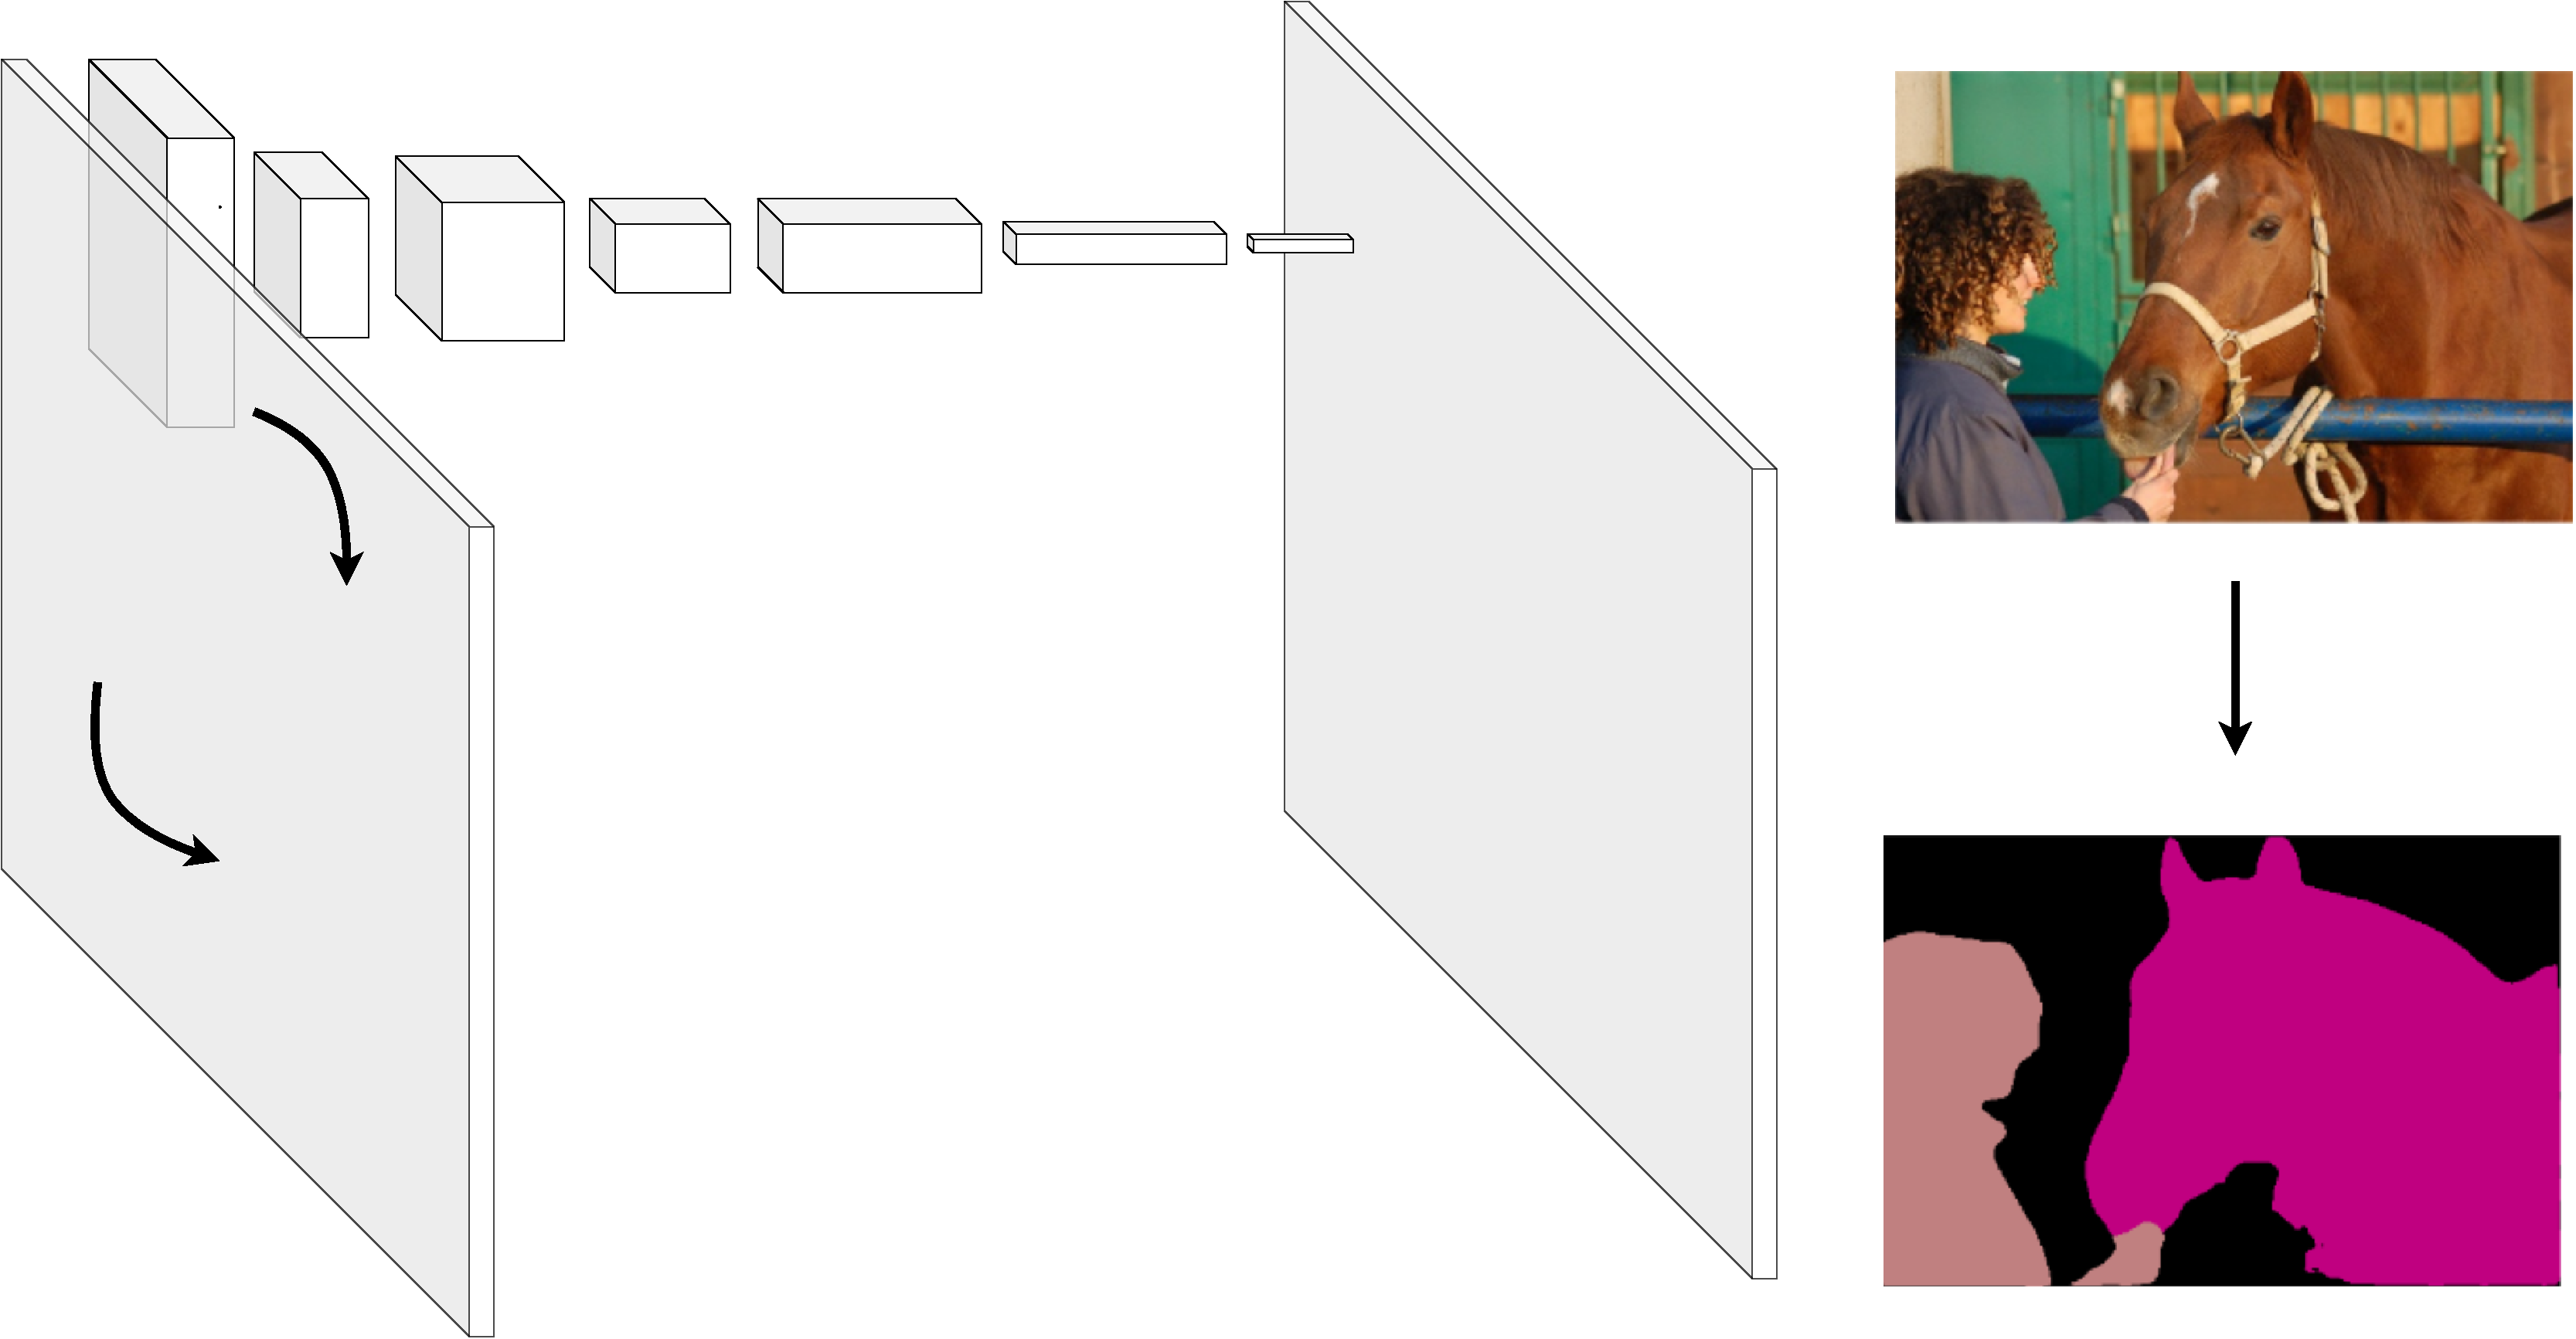
\includegraphics[width=0.9\textwidth]{segmentation_sliding_window}
  \end{figure}

  \note{
    \begin{itemize}
      \item One forward pass per pixel.
    \end{itemize}
  }
\end{frame}


\begin{frame}{Semantic Segmentation: without downsampling?}
  \begin{figure}
    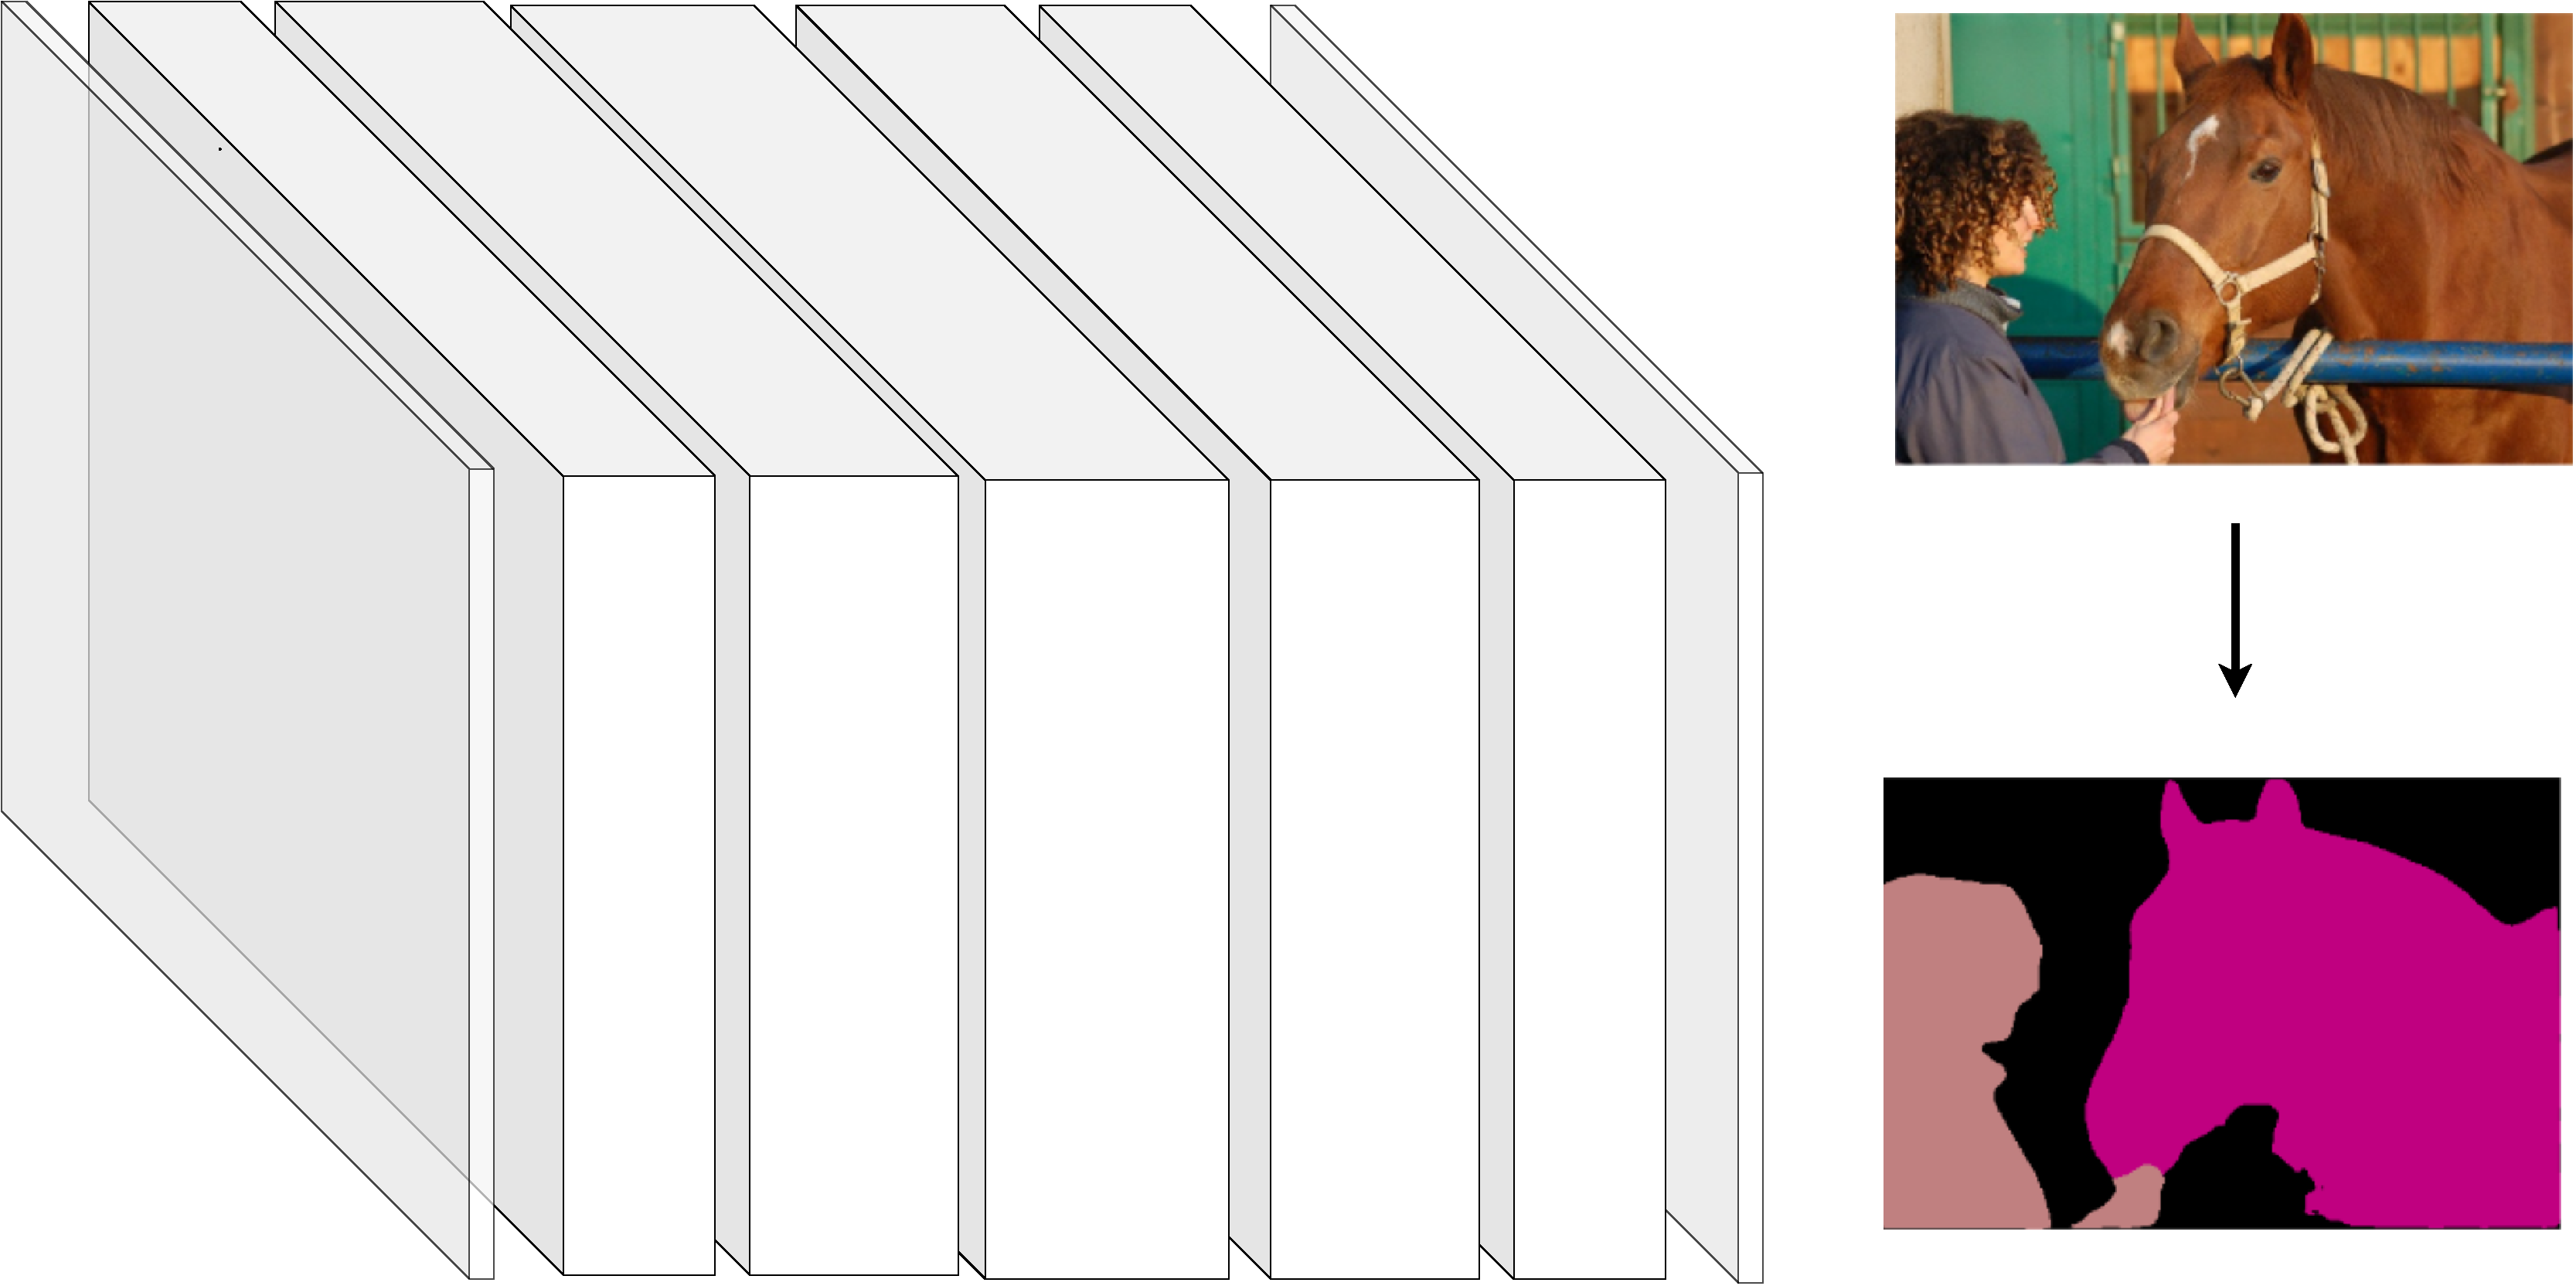
\includegraphics[width=0.9\textwidth]{segmentation_full}
  \end{figure}

  \note{
    \begin{itemize}
      \item Huge memory demands.
    \end{itemize}
  }
\end{frame}


\begin{frame}{Encoder-Decoder-Architecture}
  \begin{figure}
    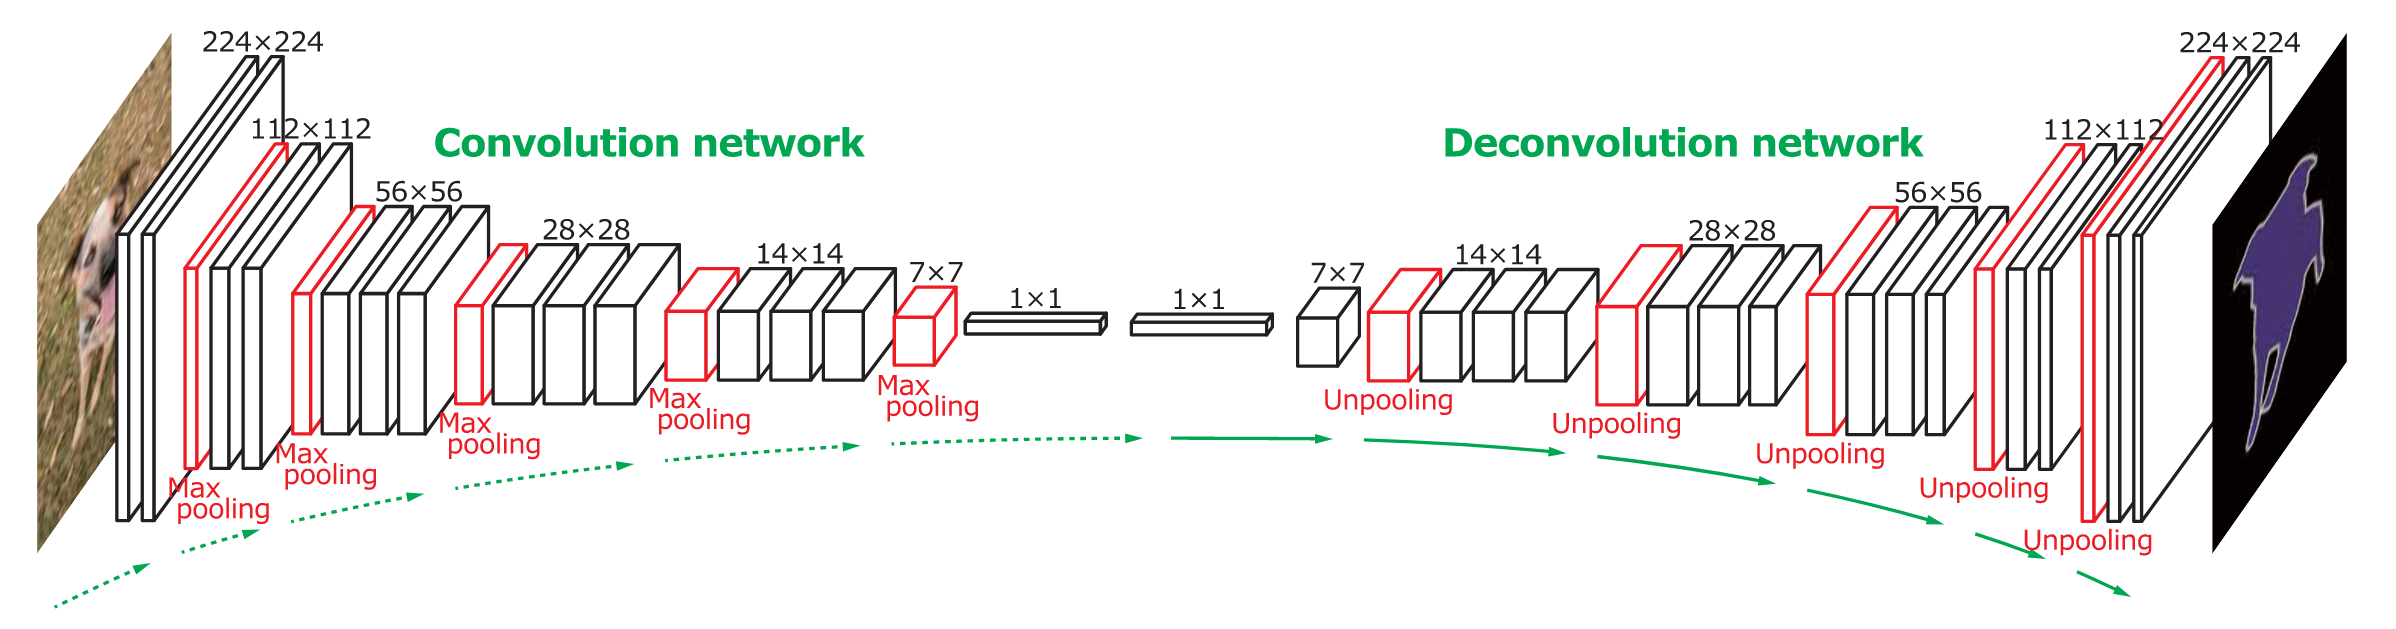
\includegraphics[width=0.9\textwidth]{encoder_decoder}
  \end{figure}
  \note{
    \begin{itemize}
      \item Image from Learning Deconvolution Network for Semantic Segmentation, Noh et al, ICCV 2015
    \end{itemize}
  }
\end{frame}


\begin{frame}{Unpooling}
  \begin{figure}
    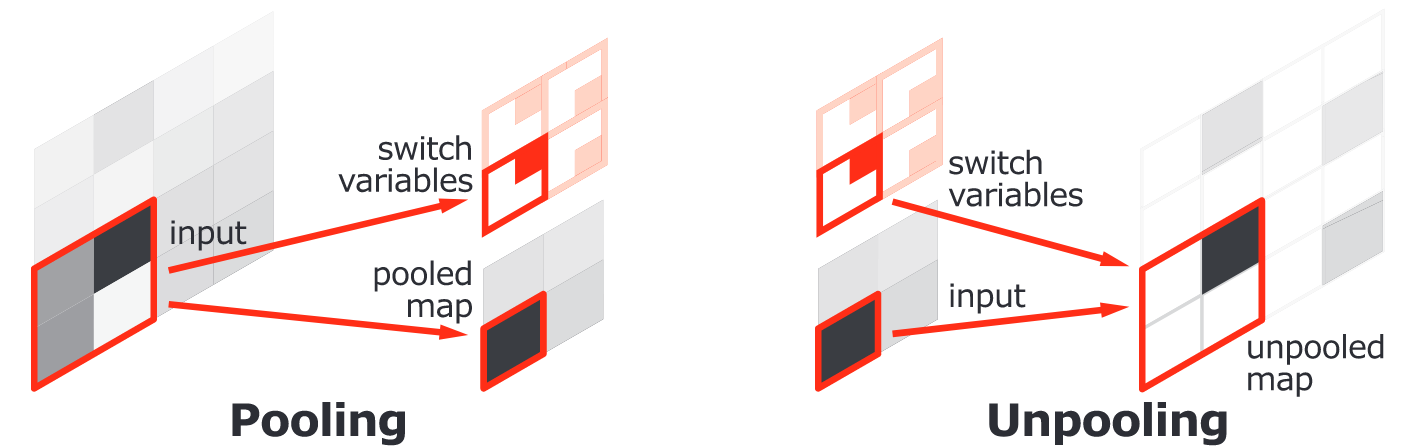
\includegraphics[width=0.9\textwidth]{pooling_unpooling}
  \end{figure}

  \note{
    \begin{itemize}
      \item Other unpooling methods: nearest neighbour or bed of nails.
      \item Image from Learning Deconvolution Network for Semantic Segmentation, Noh et al, ICCV 2015
    \end{itemize}
  }
\end{frame}


\begin{frame}{Deconvoluions}
  \begin{figure}
    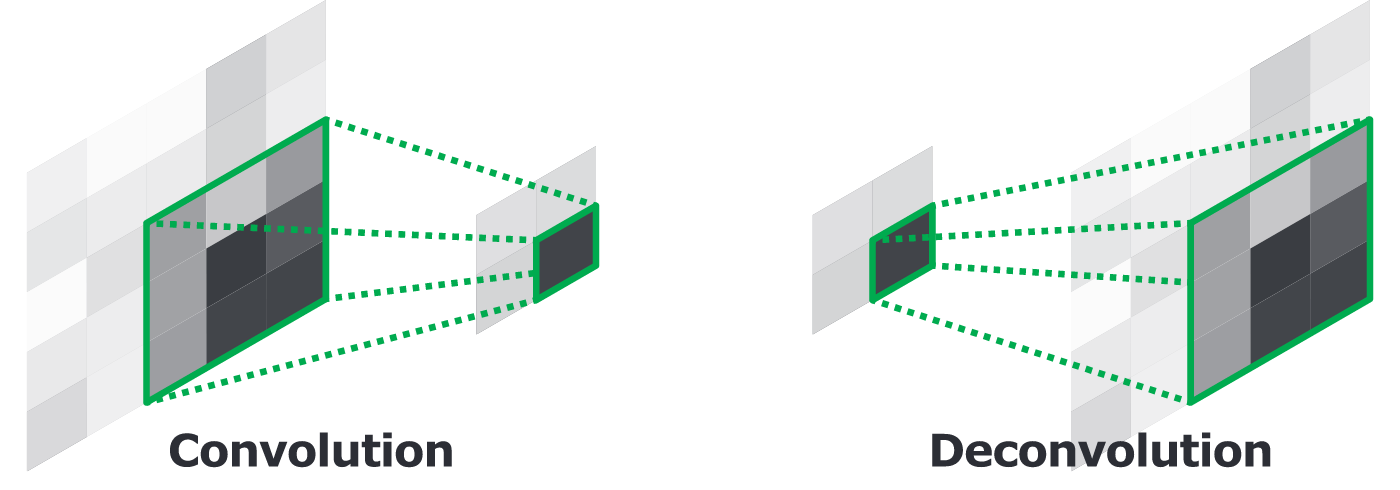
\includegraphics[width=0.9\textwidth]{conv_deconv}
  \end{figure}

  \note{
    \begin{itemize}
      \item Transpose convolution, deconvolution
      \item stride 2, pad 1, the other way
      \item Image from Learning Deconvolution Network for Semantic Segmentation, Noh et al, ICCV 2015
    \end{itemize}
  }
\end{frame}


\begin{frame}{Encoder-Decoder-Architecture}
  \begin{figure}
    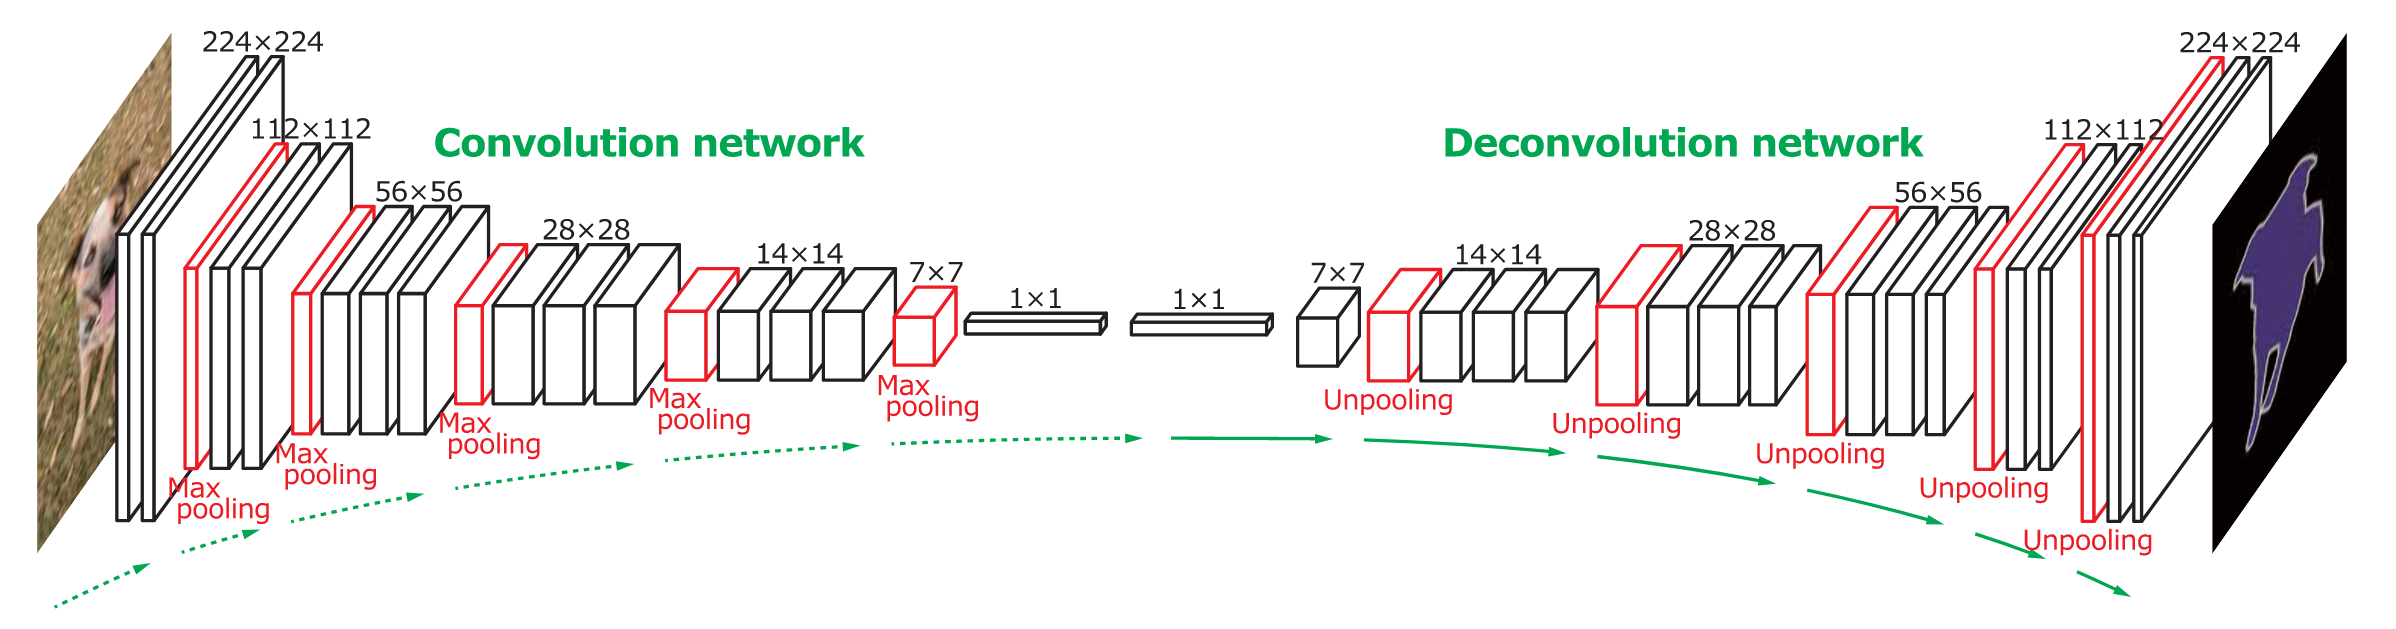
\includegraphics[width=0.9\textwidth]{encoder_decoder}
  \end{figure}
  \note{
    \begin{itemize}
      \item Problem: the coarse features (encoding in the middle) is supposed to be abstract and to not contain detailed geometrical information.
      \item Image from Learning Deconvolution Network for Semantic Segmentation, Noh et al, ICCV 2015
    \end{itemize}
  }
\end{frame}


\begin{frame}{UNet/Segnet}
  \begin{figure}
    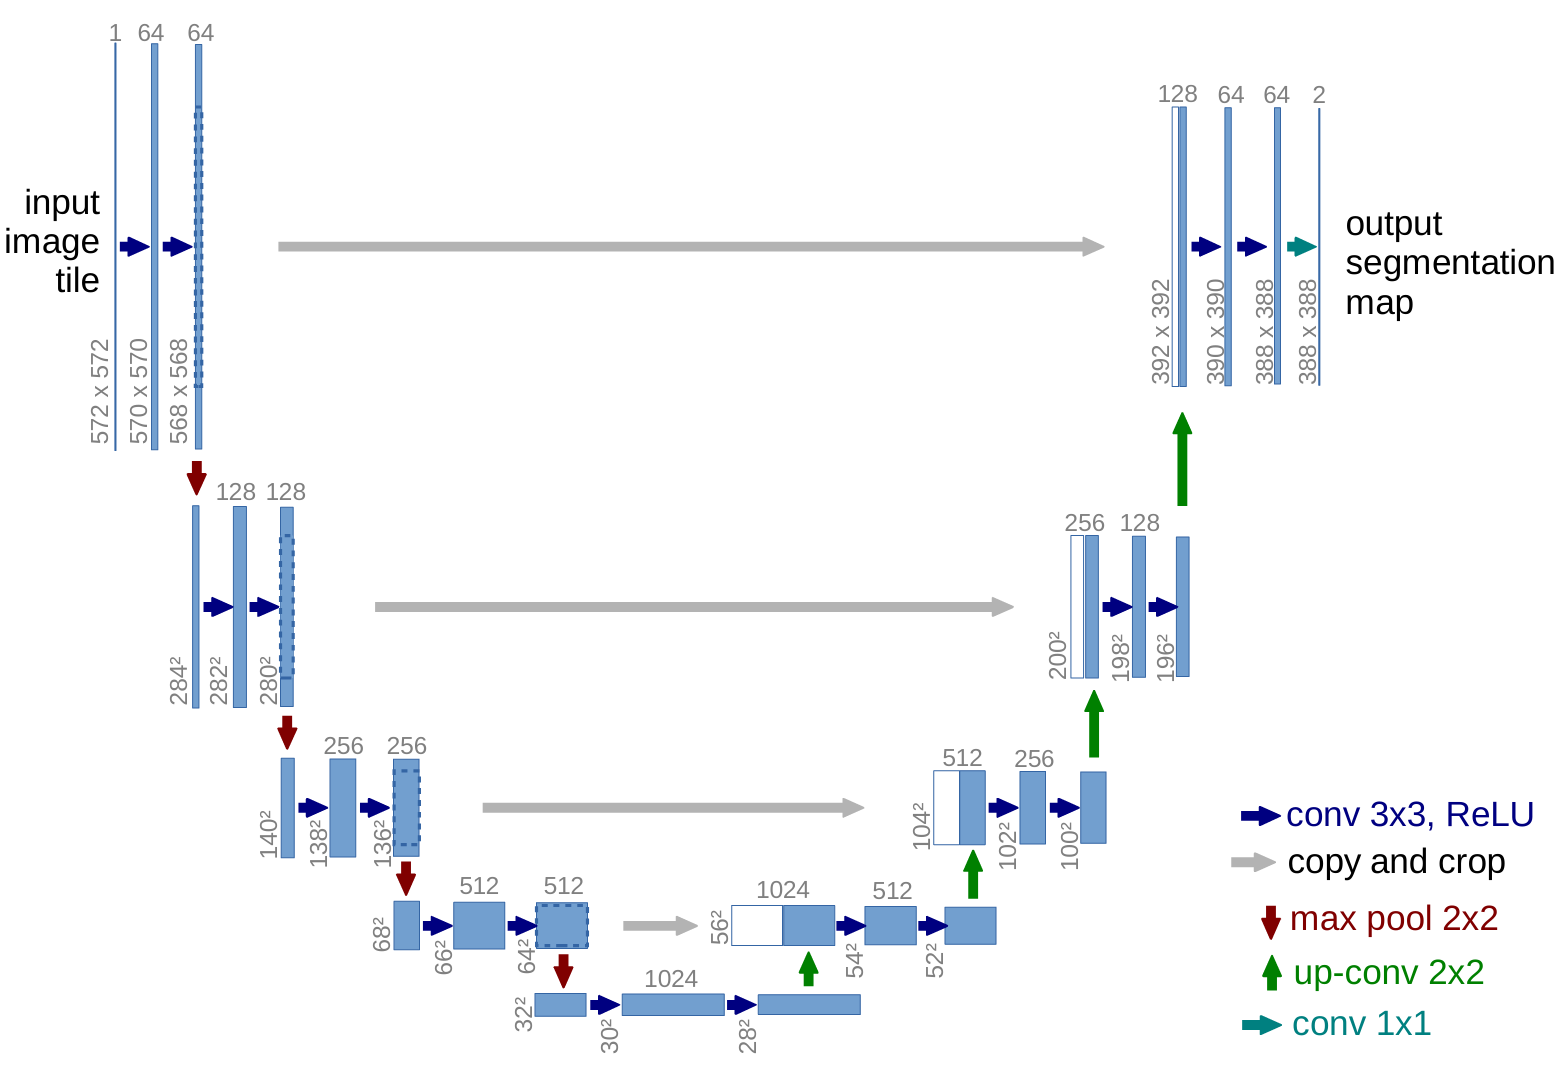
\includegraphics[width=0.55\textwidth]{unet}
  \end{figure}

  \note{
    \begin{itemize}
      \item Solution: skip connection.
      \item Image from U-Net: Convolutional Networks for Biomedical Image Segmentation, Ronnenberger et al, MICCAI 2015
      \item SegNet: A Deep Convolutional Encoder-Decoder Architecture for Image Segmentation,  Badrinarayanan et al, TPAMI 2017
    \end{itemize}
  }
\end{frame}


\begin{frame}{Pyramid Pooling}
  \begin{figure}
    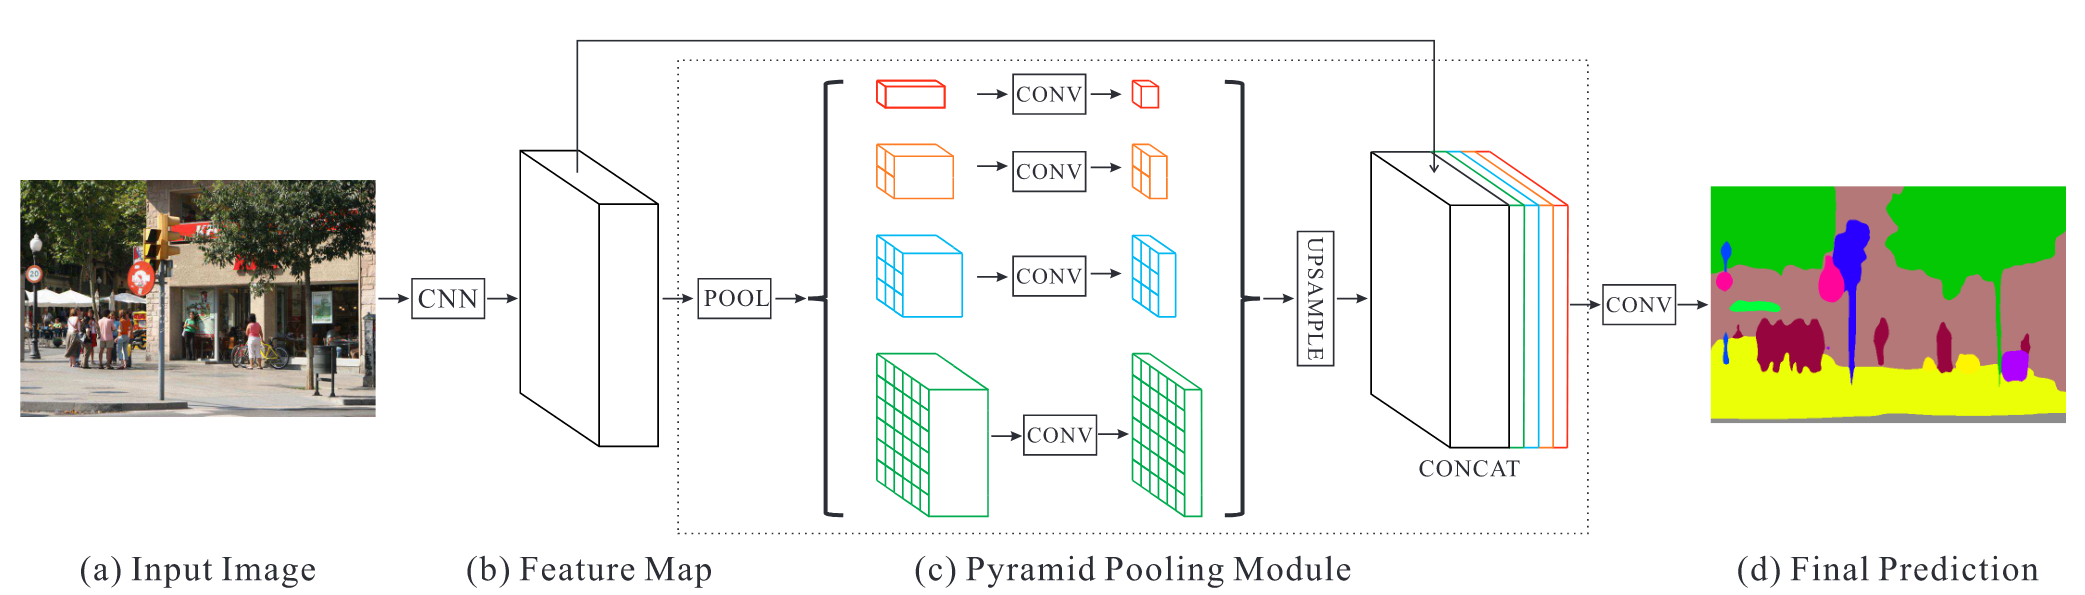
\includegraphics[width=0.9\textwidth]{pyramid_pooling}
  \end{figure}

  \note{
    \begin{itemize}
      \item Global context prior: to allow the network to process the image on different scales improves results.
      \item Improves the models ability to learn spatial semantics (spatial class co-occurence and spatial coherence).
      \item Improves recognition of very small object and stuff classes that exceed receptive fields.
      \item Image from Pyramid Scene Parsing Network, Zhao et al, CVPR 2017
    \end{itemize}
  }
\end{frame}


\begin{frame}{Pyramid Pooling: DeepLabv3+}
  \begin{figure}
    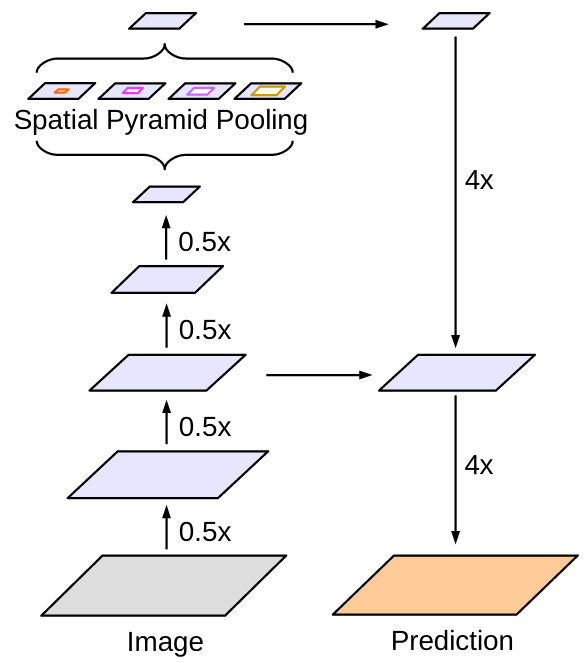
\includegraphics[width=0.45\textwidth]{deeplabv3p}
  \end{figure}

  \note{
    \begin{itemize}
      \item Case study of a SOTA semantic segmentation network: uses pretrained encoder network plus spatial pyramid pooling and skip connections.
      \item Image from Encoder-Decoder with Atrous Separable Convolution for Semantic Image Segmentation, Chen et al, ECCV 2018
    \end{itemize}
  }
\end{frame}
